\chapter{\textbf{CROCO}}
\section{Exemple de configuration de la grille verticale}
\label{sec:vertical grid}

\begin{figure}[h!]
    \centering
    \subfigure[Exemple de résolution verticale avec une résolution plus faible]{
        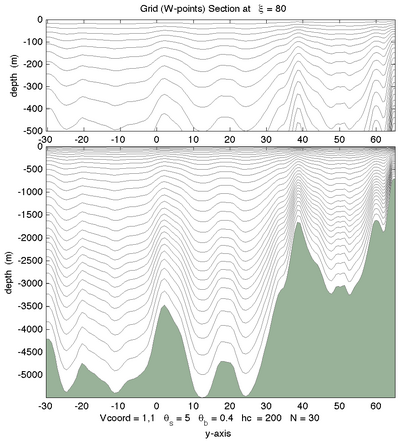
\includegraphics[width=0.45\textwidth]{figures/vcoord_ex1.png}
        \label{fig:vcoord_ex1}
    }
    \hfill
    \subfigure[Ici on a augmenté le nombre de niveaux proche de la surface et du fond de l'océan]{
        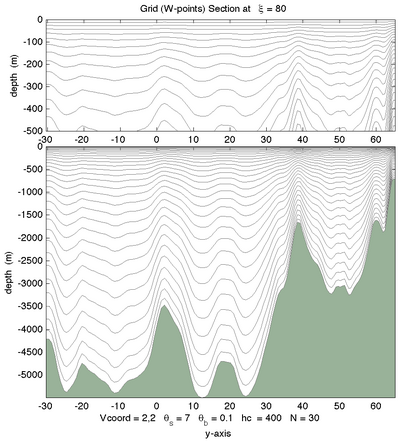
\includegraphics[width=0.45\textwidth]{figures/vcoord_ex2.png}
        \label{fig:vcoord_ex2}
    }
    \caption{Exemple de résolution verticale tiré de la documentation de \textbf{CROCO} - ROMS-RUTGERS team}
\end{figure}